% Part: sets-functions-relations
% Chapter: infinite
% Section: hilberts-hotel
%
\documentclass[../../../include/open-logic-section]{subfiles}

\begin{document}

\olfileid{sfr}{infinite}{hilbert}
\olsection{হিলবার্টের হোটেল}

স্বাভাবিক সংখ্যার সেটটি যে অসীম, তা স্পষ্ট। তাই আমরা যদি স্বাভাবিক সংখ্যাগুলিকে শুরুতেই \emph{ধরে নিতে} না চাই, তবে প্রথম কাজ হলো এমন ভাষায় অসীম সেটের বৈশিষ্ট্য নির্ধারণ করা, যেখানে স্বাভাবিক সংখ্যাগুলির নিজেদেরই উল্লেখ করতে হয় না। হিলবার্ট ১৯২৪ সালের একটি বক্তৃতায় একটি চমৎকার উপায় দেখিয়েছিলেন। তিনি আমাদের কল্পনা করতে বলেন:
\begin{quote}
[\ldots] সসীমসংখ্যক কক্ষবিশিষ্ট একটি হোটেল। এই কক্ষগুলির প্রত্যেকটিতে ঠিক একজন করে অতিথি থাকবেন। অতিথিরা এবার কোনোভাবে নিজেদের কক্ষ বদল করলেও [কিন্তু] প্রত্যেক কক্ষে যদি এখনও একজনের বেশি না থাকেন, তবে কোনো কক্ষ খালি হবে না; হোটেলের মালিক এইভাবে সদ্য আসা অতিথির জন্য নতুন কোনো স্থান তৈরি করতে পারবেন না [\ldots
\textparagraph \ldots]

এবার আমরা ধরে নিই যে হোটেলটিতে অসীমসংখ্যক ক্রমিক-সংখ্যাযুক্ত কক্ষ থাকবে—$1$, $2$, $3$, $4$, $5$, \dots—এবং প্রত্যেকটিতে ঠিক একজন করে অতিথি থাকবেন। নতুন কোনো অতিথি এলেই মালিককে শুধু পুরোনো অতিথিদের প্রত্যেককে তাঁর বর্তমান কক্ষের সংখ্যার চেয়ে এক বেশি সংখ্যার কক্ষে সরিয়ে দিতে হবে; তখন সদ্য আসা অতিথির জন্য কক্ষ~$1$ খালি হয়ে যাবে।
	\begin{center}
		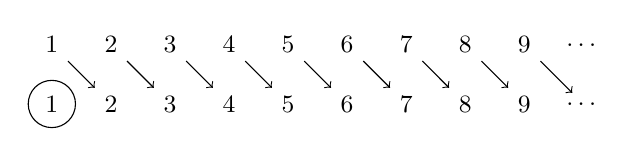
\begin{tikzpicture}[scale = .75]
		\foreach \x in {1, 2, 3, 4, 5, 6, 7, 8, 9}
		{
			\node (\x a) at (\x, 1) {\small{\x}};
			\node (\x b) at (\x, 2) {\small{\x}};
		}
		\node (dotsa) at (10, 1) {\small{\ldots}};
		\node (dotsb) at (10, 2) {\small{\ldots}};
		\draw[->] (1b)--(2a);
		\draw[->] (2b)--(3a);
		\draw[->] (3b)--(4a);
		\draw[->] (4b)--(5a);
		\draw[->] (5b)--(6a);
		\draw[->] (6b)--(7a);
		\draw[->] (7b)--(8a);
		\draw[->] (8b)--(9a);
		\draw[->] (9b)--(dotsa);
		\draw (1,1) circle (.4);
		\end{tikzpicture}
	\end{center}
	(\citealt[730]{EwaldSieg2013}-এ প্রকাশিত; অনুবাদ আমাদের)
\end{quote}
মূল কথাটি হলো, হিলবার্টের হোটেলে অসীমসংখ্যক কক্ষ আছে; এই কথাটির অর্থ নির্ধারণে আমরা তাঁর ব্যাখ্যাটিই গ্রহণ করতে পারি। বস্তুত, ডেডেকিন্ডও এই পন্থা নিয়েছিলেন (তবে এখানে অবশ্যই প্রবল কালবৈষম্যসহ উপস্থাপন করা হচ্ছে; ডেডেকিন্ডের সংজ্ঞাটি \citeyear{Dedekind1888} সালের):

\begin{defn}\ollabel{defn:DedekindInfinite}
একটি সেট $A$ \emph{ডেডেকিন্ড-অসীম} যদি এবং কেবল যদি~$A$ থেকে~$A$-এর একটি প্রকৃত উপসেটে !!a{injection} থাকে। অর্থাৎ, এমন কোনো $o \in A$ এবং !!a{injection} $f \colon A \to A$ আছে যাতে $o \notin \ran{f}$।
\end{defn}

\end{document}
